\section{Clase 14 - Pr\'actica 6 (Resoluci\'on num\'erica de ecuaciones no lineales)}

Dada una funci\'on $f$, queremos encontrar un valor $r$ tal que $f(r) = 0$. A $r$ se lo llama ra\'iz de $f$.\\

Vamos a armar una sucesi\'on de valores $x_{0}, ..., x_{n}$ de forma tal que $\lim\limits_{n \to \infty}{x_{n}} = r$.

\subsection{M\'etodo de bisecci\'on}

\begin{itemize}
    \item Tomo $[a, b]$ un intervalo tal que $f(a)f(b) < 0$

    \item Calculo $c = \frac{a + b}{2}$:\\

    Si $f(c) = 0$, ya est\'a.\\
    
    Si $f(a)f(c) > 0 \Rightarrow$ $f(a)$ y $f(c)$ tienen el mismo signo y la ra\'iz est\'a en $[c, b]$.\\
    
    Si $f(a)f(c) < 0 \Rightarrow$ $f(a)$ y $f(c)$ tienen distinto signo y la ra\'iz est\'a en $[a, c]$.\\

    \item Repito el proceso en el nuevo intervalo
\end{itemize}

\textit{Observaci\'on:} Si hay m\'as de una ra\'iz de $f$ en el intervalo $[a, b]$, este m\'etodo converger\'a a alguna de ellas.\\

Se genera una sucesi\'on de intervalos, donde cada intervalo mide la mitad del anterior:

$$[a, b] = [a_{0}, b_{0}], [a_{1}, b_{1}], ..., [a_{n}, b_{n}]$$

$$b_{n} - a_{n} = \frac{b - a}{2^{n}}$$

y una sucesi\'on

$$x_{1} = \frac{a_{0} + b_{0}}{2} \in (a_{0}, b_{0})$$
$$...$$
$$x_{n} = \frac{a_{n - 1} + b_{n - 1}}{2} \in (a_{n - 1}, b_{n - 1})$$\\

\underline{Error en el m\'etodo de bisecci\'on}

\begin{equation}
    \label{eq:err_bis}
   |r - x_{n}| \leq \frac{1}{2}(b_{n - 1} - a_{n - 1}) = \frac{b - a}{2^{n}}
\end{equation}
\\
Probamos que el m\'etodo de bisecci\'on converge a una ra\'iz $r$ de $f$, y el error en el paso n-\'esimo est\'a dado por la desigualdad (\ref{eq:err_bis}).\\

\textit{Ventajas:} es un m\'etodo muy simple de aplicar y sirve para cualquier funci\'on continua.\\

\textit{Desventajas:} es lento. No se puede generalizar a m\'as dimensiones.\\

\textit{Python}: M\'etodo de bisecci\'on\\

Elegir una funci\'on $f$ y un intervalo apropiado para utilizar el m\'etodo de bisecci\'on para aproximar una soluci\'n de la ecuación $e^{-x} = x^{2}$. Cu\'antos pasos hay que hacer para garantizar que el error sea menor que $10^{-5}$?\\

\begin{verbatim}
	import numpy as np
	import matplotlib.pyplot as plt
	
	def f(x):
	    return (np.exp(-x) - x**2)
	    
	x = np.linspace(0, 1, 50)
	
	plt.plot(x, f(x), 'b', x, np.zeros(len(x)), 'r')		
\end{verbatim}

\begin{figure}[H]
  \centering
  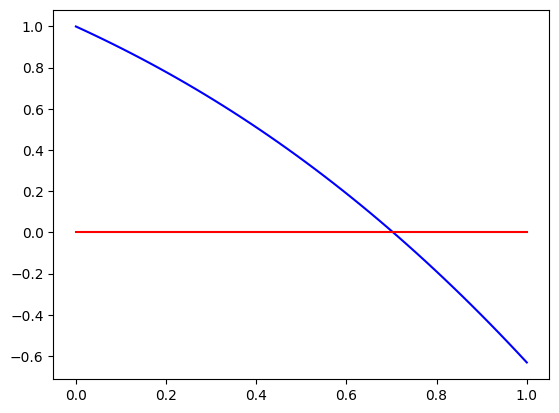
\includegraphics[width=0.6\linewidth]{Clase14_Practica6/bisect_c14p6.png}
\end{figure}

\begin{verbatim}
    def Biseccion(f, a, b, tol):
        cont = 0
        
        while (np.abs(b - a) >= tol):
            if (f(a) * f(b) > 0):
                return ('No hay raices')
            elif (f(a) * f(b) == 0):
                return ('a o b es raiz')
            else:
                c = (a + b) / 2
                cont = cont + 1
                
                print('Pasos = ', cont, 'a = ', a, 'b = ', b, 'c = ', c)
                
                if (f(c) == 0):
                    return ('c es raiz')
                else:
                    if (f(a) * f(c) < 0):
                        b = c
                    else:
                        a = c
                    
        return (a, b, c)
    
    a = 0
    b = 1
    tol = 1 * 10**(-5)
    
    a, b, c = Biseccion(f, a, b, tol)
    
    # Pasos= 1 a= 0 b= 1 c= 0.5
    # Pasos= 2 a= 0.5 b= 1 c= 0.75
    # Pasos= 3 a= 0.5 b= 0.75 c= 0.625
    # Pasos= 4 a= 0.625 b= 0.75 c= 0.6875
    # Pasos= 5 a= 0.6875 b= 0.75 c= 0.71875
    # Pasos= 6 a= 0.6875 b= 0.71875 c= 0.703125
    # Pasos= 7 a= 0.703125 b= 0.71875 c= 0.7109375
    # Pasos= 8 a= 0.703125 b= 0.7109375 c= 0.70703125
    # Pasos= 9 a= 0.703125 b= 0.70703125 c= 0.705078125
    # Pasos= 10 a= 0.703125 b= 0.705078125 c= 0.7041015625
    # Pasos= 11 a= 0.703125 b= 0.7041015625 c= 0.70361328125
    # Pasos= 12 a= 0.703125 b= 0.70361328125 c= 0.703369140625
    # Pasos= 13 a= 0.703369140625 b= 0.70361328125 c= 0.7034912109375
    # Pasos= 14 a= 0.703369140625 b= 0.7034912109375 c= 0.70343017578125
    # Pasos= 15 a= 0.70343017578125 b= 0.7034912109375 c= 0.703460693359375
    # Pasos= 16 a= 0.703460693359375 b= 0.7034912109375 c= 0.7034759521484375
    # Pasos= 17 a= 0.703460693359375 b= 0.7034759521484375 c= 0.7034683227539062	
\end{verbatim}

\subsection{M\'etodo Regula Falsi}

En vez de tomar el punto medio de $[a, b]$, tomamos la ra\'iz de la recta secante que pasa por $(a, f(a))$ y $(b, f(b))$:\\

$$\frac{f(b) - f(a)}{b - a}(x - a) + f(a) = 0 \Rightarrow x = \frac{af(b) - bf(a)}{f(b) - f(a)}$$

\begin{itemize}
    \item Tomo $[a, b]$ un intervalo tal que $f(a)f(b) < 0$

    \item Calculo $c = \frac{af(b) - bf(a)}{f(b) - f(a)}$:\\

    Si $f(c) = 0$, ya est\'a.\\
    
    Si $f(a)f(c) > 0 \Rightarrow$ $f(a)$ y $f(c)$ tienen el mismo signo y la ra\'iz est\'a en $[c, b]$.\\
    
    Si $f(a)f(c) < 0 \Rightarrow$ $f(a)$ y $f(c)$ tienen distinto signo y la ra\'iz est\'a en $[a, c]$.\\

    \item Repito el proceso en el nuevo intervalo
\end{itemize}

\subsection{M\'etodo de Newton-Raphson}

Si $f$ es derivable, en vez de tomar la ra\'iz de la recta secante, tomamos la ra\'iz de la recta tangente. ¿C\'omo?\\

$$x_{0} \rightarrow f'(x_{0})(x - x_{0}) + f(x_{0}) = 0 \rightarrow x_{1} = x_{0} - \frac{f(x_{0})}{f'(x_{0})}$$

si $f'(x_{0}) \neq 0$. Siguiendo con la iteraci\'on

$$f'(x_{1})(x - x_{1}) + f(x_{1}) = 0\ ...$$

\begin{itemize}
    \item Tomo $x_{0} \in [a, b]$

    \item Para $n = 0, 1, 2, ...$, $x_{n + 1} = x_{n} - \frac{f(x_{n})}{f'(x_{n})}$
\end{itemize}

Este m\'etodo no siempre converge.\\

\underline{Error en el m\'etodo de Newton-Raphson}\\

Llamemos $e_{n} = x_{n} - r$. Por Taylor:

$$0 = f(r) = f(x_{n}) + f'(x_{n})(r - x_{n}) + \frac{f''(\theta_{n})}{2}(r - x_{n})^{2}$$

con $\theta$ entre $r$ y $x_{n}$.\\

Despejando, $f'(x_{n})(x_{n} - r) - f(x_{n}) = \frac{f''(\theta_{n})}{2}e_{n}^{2}$. Entonces, diviendo por $f'(x_{n})$:\\

$$x_{n} - r - \frac{f(x_{n})}{f'(x_{n})} = \frac{f''(\theta_{n})}{2f'(x_{n})}e_{n}^{2} \Rightarrow x_{n + 1} - r = \frac{f''(\theta_{n})}{2f'(x_{n})}e_{n}^{2}$$\\

Nos queda:

$$e_{n + 1} = \frac{f''(\theta_{n})}{2f'(x_{n})}e_{n}^{2}$$\\

Debemos pedir $f$ con derivadas hasta orden 2 continuas y $f' \neq 0$. Notemos que, si el m\'etodo converge,\\

$$\frac{e_{n + 1}}{e_{n}} = \frac{f''(\theta_{n})}{2f'(x_{n})} \rightarrow \frac{f''(r)}{2f'(r)} < \infty$$\\

lo hace con orden (al menos) 2.\\

Casos de convergencia para todo $x_{0}$ inicial:

\begin{itemize}
    \item $f' > 0, f'' > 0$ en todo $\mathbb{R}$
    \item $f' > 0, f'' < 0$ en todo $\mathbb{R}$
    \item $f' < 0, f'' > 0$ en todo $\mathbb{R}$
    \item $f' < 0, f'' < 0$ en todo $\mathbb{R}$
\end{itemize}

\subsubsection{Convergencia local del m\'etodo de Newton-Raphson}

Si $f$ tiene dos derivadas continuas en $[a, b], f(r) = 0, f'(r) \neq 0, r \in (a, b)$. Entonces, existe $[c, d] \subseteq [a, b]$ con $r \in [c, d]$ tal que si $x_{0} \in [c, d]$, entonces el m\'etodo converge a $r$. ¿C\'omo encuentro $[c, d]$?\\

Consideramos un intervalo $I \subseteq [a, b]$ tal que $r \in I$ (lo puedo verificar por Bolzano) y adem\'as

$$max_{z \in I} |f''(z)| \leq M$$
$$min_{z \in I} |f'(z)| \geq m$$\\

Sea $L$ tal que $\frac{M}{2m}L < 1$ (o sea $L < \frac{2m}{M}$) y consideramos $[c, d]$ tal que

$$r \in [c, d]$$
$$d - c \leq L$$
$$[c - L, d + L] \subseteq I$$\\

Veamos: si $x_{0} \in [c, d] \Rightarrow |e_{0}| \leq L$ y como $|f''(z)| \leq M, |f'(z)| \geq m\ \forall z \in [c, d]$,

$$|e_{1}| = \frac{f''(\theta_{n})}{2f'(x_{0})}|e_{0}|^{2} \leq \frac{M}{2m}|e_{0}||e_{0}| \leq \frac{M}{2m}L|e_{0}| = \lambda|e_{0}|$$\\

Como $\lambda < 1$, tenemos $|e_{1}| < |e_{0}| < L$ y $x_{1} \in I$, $\theta_{1} \in I$

$$|e_{2}| = \frac{f''(\theta_{n})}{2f'(x_{1})}|e_{1}|^{2} \leq \frac{M}{2m}|e_{1}||e_{1}| \leq \frac{M}{2m}L|e_{1}| = \lambda|e_{1}| \leq \lambda^{2}|e_{0}$$
$$ ... $$
$$ |e_{n}| \leq \lambda^{n}|e_{0}|$$\\

Como $\lambda < 1$, tenemos $\lim\limits_{n \to \infty}{|e_{n}|} = 0$.\\

\textit{Python}: M\'etodo de Newton - Raphson\\

Utilizar el m\'etodo de Newton - Raphson con $x_{0} = 0$ para aproximar la soluci\'on de la ecuaci\'on $e^{-x} = x^{2}$ en el intervalo $[0, 1]$. Analizar la convergencia.\\

\begin{verbatim}
	import numpy as np
	import matplotlib.pyplot as plt
	
	def f(x):
	    return (np.exp(-x) - x**2)
	    
	x = np.linspace(0, 1, 50)
	
	plt.plot(x, f(x), 'b', x, np.zeros(len(x)), 'r')		
\end{verbatim}

\begin{figure}[H]
  \centering
  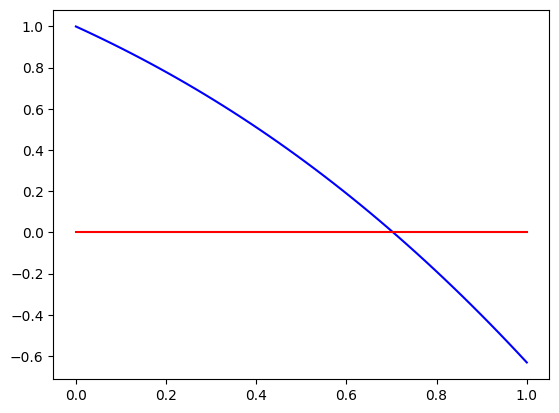
\includegraphics[width=0.6\linewidth]{Clase14_Practica6/bisect_c14p6.png}
\end{figure}

\begin{verbatim}
    def Derf(x):
        return (-1 * np.exp(-x) - 2 * x)
        
    def Newton(f, Derf, x0, MaxIter, tol):
        x1 = x0 - (f(x0) / Derf(x0))
        
        i = 1
        
        while ((i < MaxIter) and (np.abs(x0 - x1) > tol)):
            i = i + 1
            x0 = x1
            x1 = x0 - (f(x0) / Derf(x0))
            
            print('i = ', i, 'x1 = ', x1)
            
        return (i, x1)
        
    x0 = 0
    MaxIter = 100
    tol = 1 * 10**(-5)
    
    i, x1 = Newton(f, Derf, x0, MaxIter, tol)
    
    # i = 2 x1 = 0.7330436052454454
    # i = 3 x1 = 0.703807786324133
    # i = 4 x1 = 0.7034674683317975
    # i = 5 x1 = 0.7034674224983924
    
    # Probamos con otra semilla
    x0 = -500
    MaxIter = 1000
    
    i, x1 = Newton(f, Derf, x0, MaxIter, tol)

    # i = 2 x1 = -498.0
    # i = 3 x1 = -497.0
    # i = 4 x1 = -496.0
    # ...
    # i = 505 x1 = 0.703467440228491
    # i = 506 x1 = 0.7034674224983918
\end{verbatim}